\subsection{Clasificación de imágenes para localización}

Para completar la arquitectura CloudNAO falta implementar un modelo de aprendizaje 
profundo que se brinde como un servicio web para ser consumido por robots NAO.
A pesar de que el servicio de detección de objetos es mantenido por el LAR, y 
se adaptó para ser consumido a través de la API REST, no fue construido
desde cero ya que es parte de la API de detección de objetos de TensorFlow.
Es por eso que como parte final del proyecto se desarrolló un modelo para que 
resuelva la tarea de clasificar imágenes.

El problema de clasificación de imágenes es la tarea de asignarle a una imagen de
entrada una etiqueta a partir de un conjunto de categorías. Este es uno de los principales
problemas dentro del campo de la visión computacional, que a pesar de su simplicidad
tiene bastantes aplicaciones prácticas. Entre esas aplicaciones, muchas interesan al
campo de la robótica móvil, por ejemplo, para la navegación de un robot de manera
autónoma, nos gustaría que supiera en que lugar está simplemente con una fotografía
que obtenga en ese momento desde sus cámaras, así podría saber si ha llegado al 
lugar de su objetivo, o a partir de la zona donde se ubica planear una trayectoria.

Lo anterior nos inspiró en la creación de un modelo que clasificara imágenes
de algunos lugares sobre los que podría navegar el robot NAO. 
Como solución a este problema de clasificación se propuso usar 
una red neuronal convolucional, que recibiera como entrada un arreglo con los
pixeles de una imagen tomada por el robot, y la salida fuera la categoría
a la que pertenece esa imagen. 
Las clases en las que se desea clasificar las imágenes son lugares alrededor
del Laboratorio de Algoritmos para la Robótica, que se ubica en el cubículo $15$ del
Centro de Desarrollo Tecnológico de la FES Acatlán. Se eligieron las siguientes cuatro zonas:

\begin{itemize}
    \item El cubículo.
    \item La salida de emergencia.
    \item La cancha de entrenamiento de fútbol para el robot NAO.
    \item Zona de trabajo del Laboratorio.
\end{itemize}

Para finalizar,
se debe integrar uno de los cinco modelos descritos en la tabla \ref{table:models_results} sobre la API REST de CloudNAO y luego hacer peticiones con el robot a ésta.
Los modelos elaborados en TensorFlow contienen la gráfica de cómputo
y los valores de los parámetros que se han entrenado. Estos datos
están contenidos en varios archivos que se pueden guardar para
entrenamientos posteriores o para realizar inferencias sobre 
un modelo cuyas variables han sido aprendidas.

Se eligió el modelo con la precisión más alta y con el menor
tiempo de entrenamiento que es el modelo (1). 
%Durante la ejecución
%de la gráfica del modelo se crea una instancia de la clase \texttt{tf.train.Saver()}. Esto crea cuatro archivos
%uno con extensión \texttt{.meta}, uno con extensión \texttt{.index},
%otro con extensión \texttt{.data} y otro sin extensión llamado
%\texttt{checkpoint}. El primero guarda toda la gráfica de
%TensorFlow, los otros tres almacenan los valores de las variables.
%Después de guardar, simplemente se restaura el modelo
%y se puedan hacer inferencias al alimentarlo con una imagen.
Dentro de la API REST, la clase que se encarga de restaurar la gráfica y valores del modelo
es \texttt{ImageClasssfier} dentro del módulo \texttt{indoor\_scenes\_classsifier} del paquete \texttt{tf\_models}.
En el apartado \textit{Modelos de TensorFlow (tf\_models)}
de la sección \ref{chapter_two/desc_cloudnao:api-rest-de-cloudnao}
se describe cómo utilizar esta clase.

Por otra parte el robot NAO o cualquier otro
dispositivo cliente se comunica con la API a través
de una biblioteca que permita hacer peticiones 
HTTP. En el caso del robot ocupamos la biblioteca
\texttt{requests} de Python. Para obtener una imagen 
del robot codificada en base 64 se utilizó la clase \texttt{Robot}
del módulo \texttt{nao\_robot} descrito en la sección
\ref{\detokenize{firebase-nao-robot}}. Es la cadena
que representa la imagen la que se envía a la API REST usando
\texttt{requests}.

Se hicieron $40$ solicitudes a la API REST desde el robot,
$10$ por cada categoría. Esto es, se enviaron
$10$ imágenes de la cancha, $10$ de la salida,
$10$ del cubículo y $10$ del área de trabajo.
En las tablas \ref{table:soccer_nao_results},
\ref{table:exit}, \ref{table:desks} y
\ref{table:office}, se resumen los resultados obtenidos.
En la figura \ref{nao_api_images} se muestran algunas imágenes capturadas en las pruebas.



Se puede ver que existen más aciertos
con imágenes de la cancha de fútbol, 8 de 10 inferencias correctas.
Clasificando imágenes de la salida de emergencia
y del cubículo se tienen 7 de 10 predicciones correctas.
Para el área de trabajo tuvo su peor desempeño con 6 de
10 aciertos. Si bien no se obtiene
la precisión reportada durante el
entrenamiento del modelo, el tiempo
de ejecución y los
resultados son buenos
para la funcionalidad de
auxiliar a la navegación del robot.
El tiempo de solicitud y repuesta varía entre peticiones.
Factores que influyen al tiempo son el tamaño de la 
imagen enviada y la velocidad de la conexión del cliente
y del servidor. Convendría probar el modelo sobre PaaS
como Google Cloud o Heroku para ver si hay una mejora
en el tiempo.



\begin{table}[!h]
\centering
\begin{tabular}{|l|l|l|l|}
\hline
Clase        & Predicción   & Tiempo        & Correcta \\ \hline
cancha & z. trabajo        & 3.0337650776 & F        \\ \hline
cancha & cancha & 3.0559039116 & T        \\ \hline
cancha & z. trabajo        & 2.09687018394 & F        \\ \hline
cancha & cancha & 3.0169699192 & T        \\ \hline
cancha & z. trabajo        & 2.32713413239 & F        \\ \hline
cancha & cancha & 3.0284428596 & T        \\ \hline
cancha & cancha & 3.0252449512 & T        \\ \hline
cancha & cancha & 3.1204240322 & T        \\ \hline
cancha & cancha & 3.013076067  & T        \\ \hline
cancha & cancha & 3.2163701057 & T        \\ \hline
\end{tabular}
\caption{Resultados de las imágenes de la cancha de fútbol.}
\label{table:soccer_nao_results}
\end{table}

\begin{table}[!h]
\centering
\begin{tabular}{|l|l|l|l|}
\hline
Clase & Predicción & Tiempo        & Correcta \\ \hline
salida  & salida       & 3.2262349129 & T     \\ \hline
salida  & salida       & 3.0402858257 & T     \\ \hline
salida  & salida     & 3.298979044  & T    \\ \hline
salida  & cubículo     & 3.6488580704 & F    \\ \hline
salida  & salida       & 3.4767799377 & T     \\ \hline
salida  & salida       & 3.6147930622 & T     \\ \hline
salida  & salida       & 3.7430388927 & T     \\ \hline
salida  & cubículo     & 3.7496609688 & F    \\ \hline
salida  & salida       & 3.8713350296 & T     \\ \hline
salida  & cubículo     & 4.0420210361 & F    \\ \hline
\end{tabular}
\caption{Resultados para fotografías de la salida de emergencia.}
\label{table:exit}
\end{table}

\begin{table}[!h]
\centering
\begin{tabular}{|l|l|l|l|}
\hline
Clase      & Predicción & Tiempo        & Correcta \\ \hline
z. trabajo & z. trabajo & 5.3504459858 & T        \\ \hline
z. trabajo & cubículo    & 5.2893049717 & F        \\ \hline
z. trabajo & cubículo    & 5.2149860859 & F        \\ \hline
z. trabajo & z. trabajo & 5.2179970741 & T        \\ \hline
z. trabajo & cubículo    & 5.6882929802 & F        \\ \hline
z. trabajo & cubículo    & 5.6848390102 & F        \\ \hline
z. trabajo & z. trabajo & 5.9792921543 & T        \\ \hline
z. trabajo & z. trabajo & 5.8859920502 & T        \\ \hline
z. trabajo & z. trabajo & 5.722206831  & T        \\ \hline
z. trabajo & z. trabajo & 6.7581658363 & T        \\ \hline
\end{tabular}
\caption{Resultados para la fotografías del área
de trabajo.}
\label{table:desks}
\end{table}

\begin{table}[!h]
\centering
\begin{tabular}{|l|l|l|l|}
\hline
Clase   & Predicción & Tiempo        & Correcta \\ \hline
cubículo & cubículo    & 3.5342819691 & T        \\ \hline
cubículo & cubículo    & 3.9999611378 & T        \\ \hline
cubículo & z. trabajo & 4.6536300182 & F        \\ \hline
cubículo & z. trabajo & 3.8637499809 & F        \\ \hline
cubículo & z. trabajo & 4.887745142  & F        \\ \hline
cubículo & cubículo    & 4.4888358116 & T        \\ \hline
cubículo & cubículo    & 4.6198430061 & T        \\ \hline
cubículo & cubículo    & 4.4448840618 & T        \\ \hline
cubículo & cubículo    & 4.5735599995 & T        \\ \hline
cubículo & cubículo    & 5.2998209    & T        \\ \hline
\end{tabular}
\caption{Resultados de obtenidos con imágenes del cubículo.}
\label{table:office}
\end{table}

\begin{figure}[!ht] 
  \centering
\subfloat[Clase = cancha, predicción = cancha. Tiempo = 3.05]{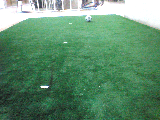
\includegraphics[scale=1]{nao_api_soccer}}
\qquad
\subfloat[Clase = salida, predicción = salida. Tiempo = 3.29]{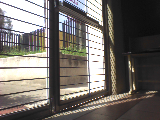
\includegraphics[scale=1]{exit_incorrect}}
\qquad
\subfloat[Clase = zona de trabajo, predicción = cubículo. Tiempo = 5.21]{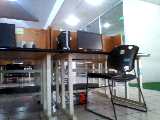
\includegraphics[scale=1]{deks_incorrect}}
\qquad
\subfloat[Clase = cubículo, predicción = cubículo. Tiempo = 3.53]{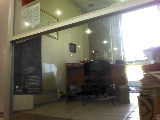
\includegraphics[scale=1]{nao_api_office}}
\caption{Predicciones hechas enviando imágenes del robot a la API REST. El tiempo son los
segundos que se tardó en enviar la solicitud y en recibir la respuesa. \label{nao_api_images}}
\end{figure}
